\section{OpenSWATH for Metabolomics}
\subsection{Introduction}
We would like to present an automated DIA/SWATH analysis workflow for metabolomics, which takes advantage of experiment specific target-decoy assay library generation. This allows for targeted extraction, scoring and statistical validation of metabolomics DIA data \cite{Rost2014}, \cite{Teleman2015}. 

\subsection{Workflow}

The workflow follows multiple steps (see Fig. \ref{fig:pipline_overview}). 

\paragraph{Candidate identification} Feature detection, adduct grouping and accurate mass search are applied on DDA data. 
\paragraph{Library construction}  The knowledge determined from the DDA data, about  compound identification, its potential adduct and the corresponding fragment spectra are used to perform fragment annotation via compositional fragmentation trees \cite{Duhrkop2019}. Afterwards transitions, which are the reference of a precursor to its fragment ions are stored in a so-called assay library. Assay libraries usually contain additional metadata (i.e. retention time, peak intensities). FDR estimation is based on the target-decoy approach \cite{Elias2007}. For the generation of the MS2 decoys, the fragmentation tree-based rerooting method ensures the consistency of decoy spectra \cite{Scheubert2017}. Targeted extraction - The target-decoy assay library is then used to analyse SWATH data. 
\paragraph{Targeted extraction} Chromatogram extraction and peak-group scoring. This step is performed using an algorithm based on OpenSWATH \cite{Rost2014} for metabolomics data. 
\paragraph{Statistical validation} FDR estimation uses the PyProphet algorithm \cite{Teleman2015}. To prevent overfitting we chose the simpler linear model (LDA) for target-decoy discrimination in PyProphet, using MS1 and MS2 scoring with low correlated scores.

\begin{figure}[!t]
  \centering
  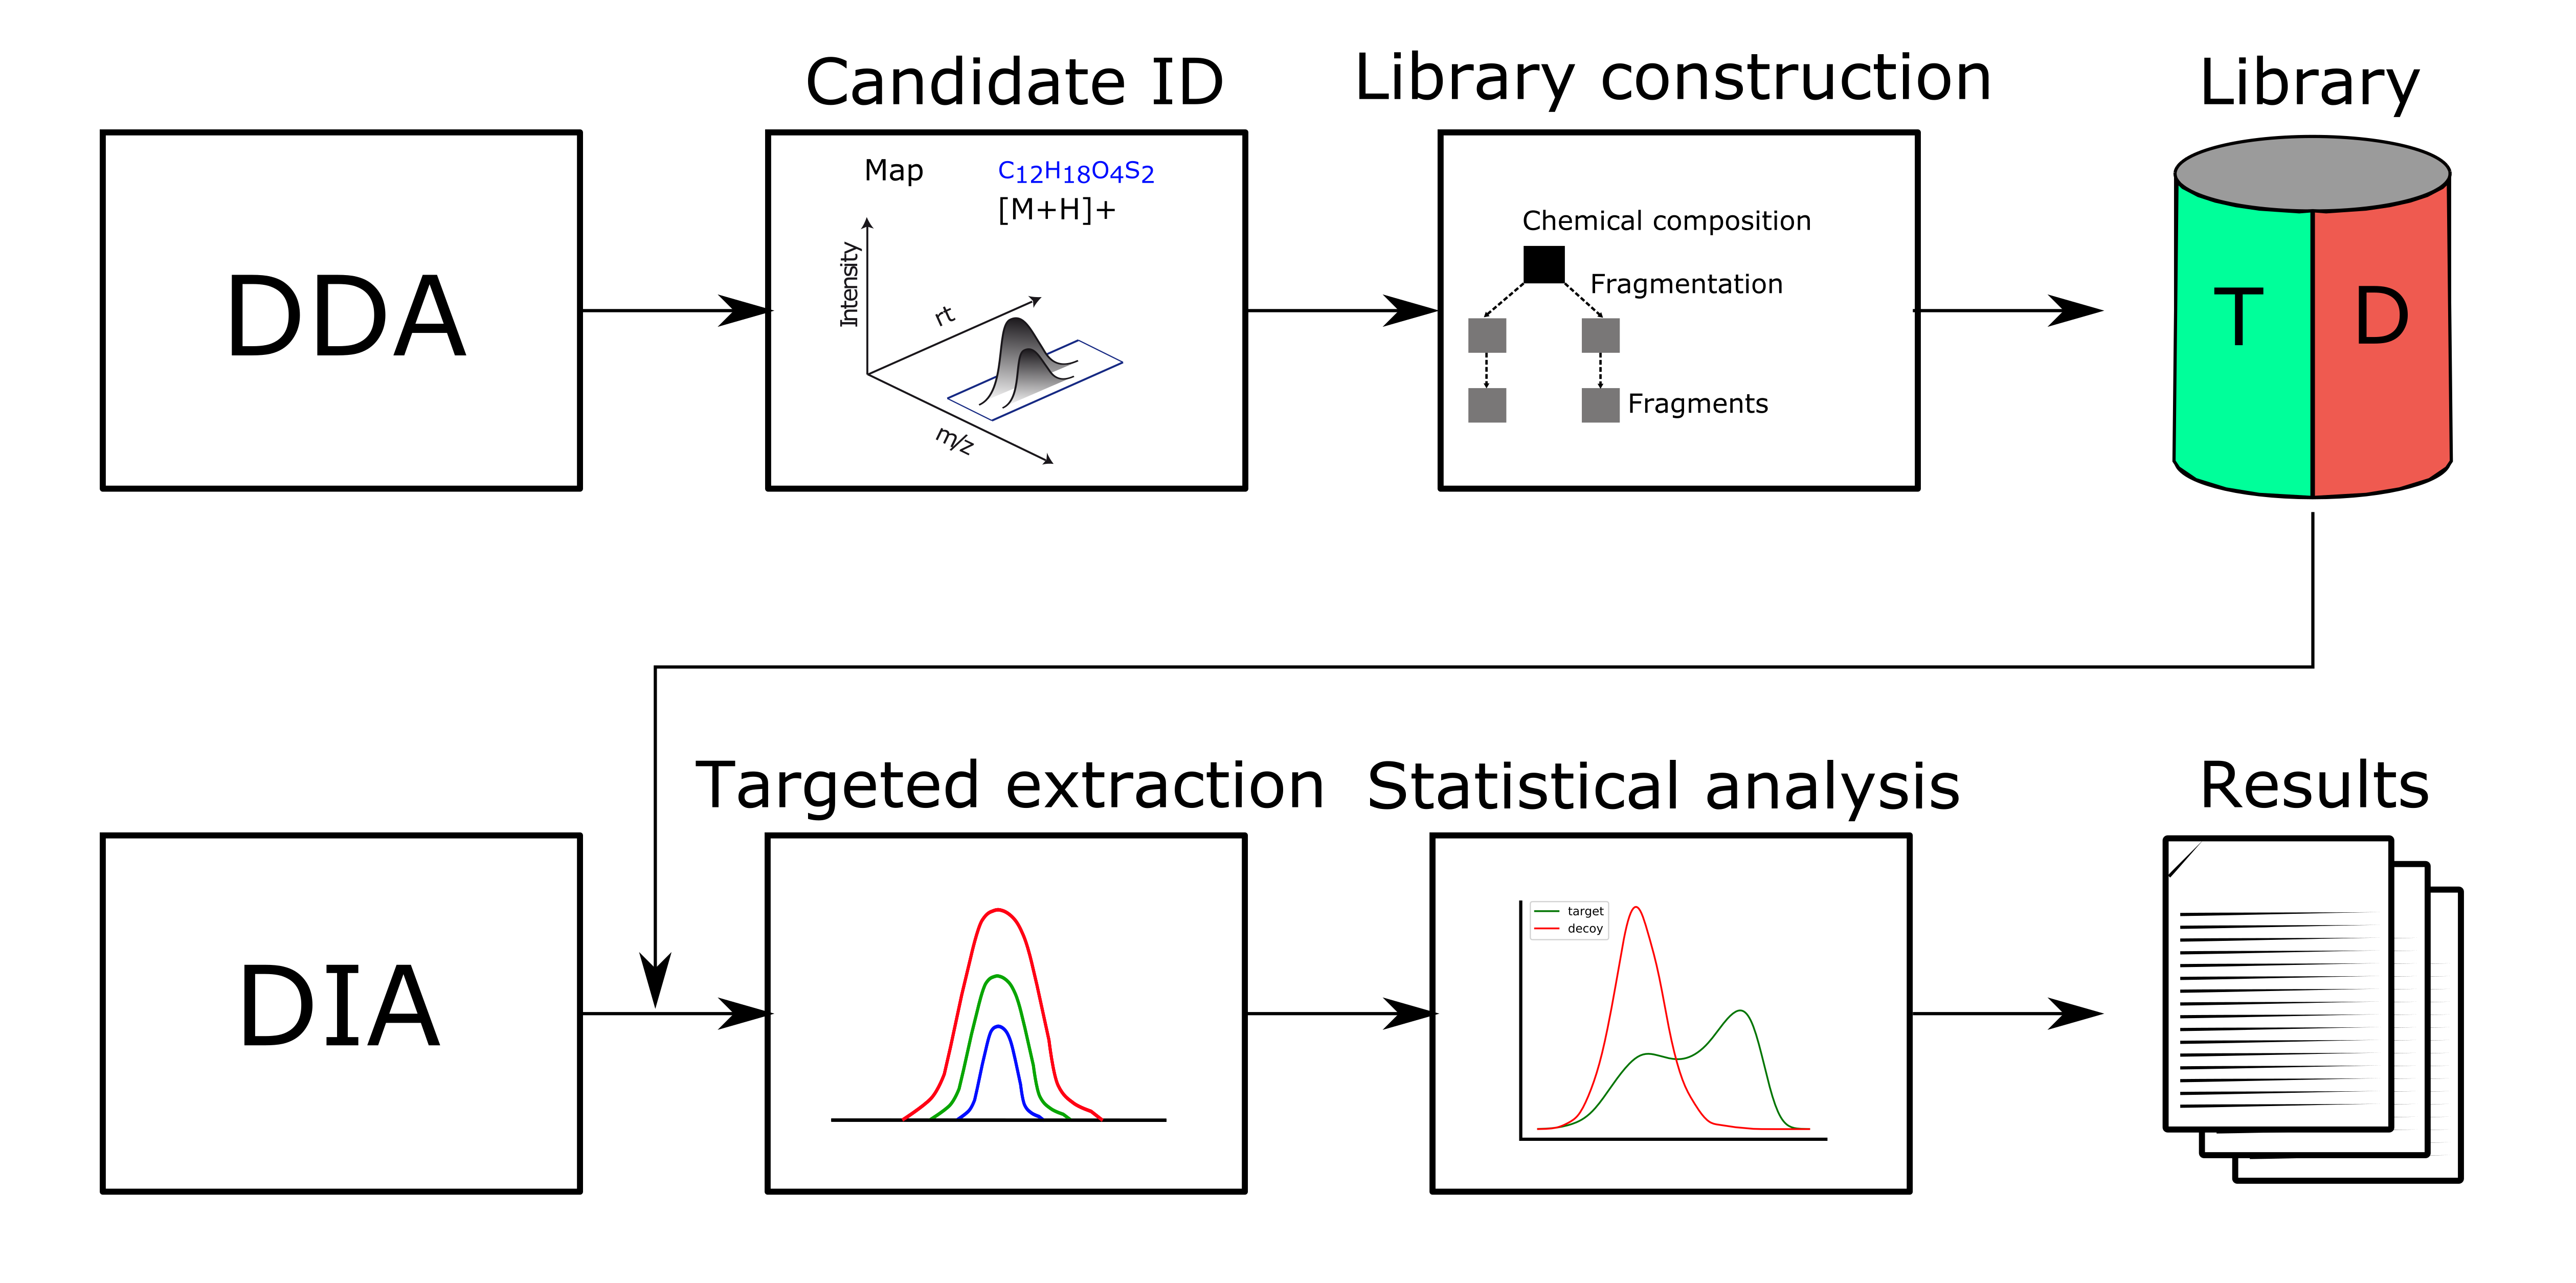
\includegraphics[width=0.7\textwidth]{graphics/openswathmetabo/pipeline_overview.png}
  \caption{DIAMetAlyzer - pipeline for assay library generation and targeted analysis with statistical validation. DDA data is used for candidate identification containing feature detection, adduct grouping and accurate mass search. Library construction uses fragment annotation via compositional fragmentation trees and decoy generation using a fragmentation tree re-rooting method to create a target-decoy assay library. This library is used in a second step to analyse metabolomics DIA data performing targeted extraction, scoring and statistical validation (FDR estimation).}
  \label{fig:pipline_overview}
\end{figure}

\subsection{Prerequisites}
Apart from the usual KNIME nodes, the workflow uses python scripting nodes. One basic requirement for the installation of python packages, in particular pyOpenMS, is a package manager for python. Using conda as an environment manger allows to specify a specific environment in the KNIME settings (\menu{File -> Preferences -> KNIME -> Python})

\subsubsection{Windows}
We suggest do use a virtual environment for the Python 3 installation on windows. 
Here you can install miniconda and follow the further instructions. \\

\begin{enumerate}
  \item Create new conda python environment
    \begin{lstlisting}
    conda create -n py37 python=3.7
    \end{lstlisting} 
    \item Activate py37 environment
    \begin{lstlisting}
    conda activate py37
    \end{lstlisting} 
  \item Install pip (see above)
  \item On the command line:
    \begin{lstlisting}
    python -m pip install -U pip
    python -m pip install -U numpy
    python -m pip install -U pandas
    python -m pip isntall -U pyprophet
    python -m pip install -U pyopenms
    \end{lstlisting}
\end{enumerate}

\subsubsection{MacOS}
We suggest do use a virtual environment for the Python 3 installation on Mac. 
Here you can install miniconda and follow the further instructions. \\

\begin{enumerate}
  \item Create new conda python environment
    \begin{lstlisting}
    conda create -n py37 python=3.7
    \end{lstlisting} 
    \item Activate py37 environment
    \begin{lstlisting}
    conda activate py37
    \end{lstlisting} 
  \item On the Terminal:
    \begin{lstlisting}
    python -m pip install -U pip
    python -m pip install -U numpy
    python -m pip install -U pandas
    python -m pip isntall -U pyprophet
    python -m pip install -U pyopenms
    \end{lstlisting}
\end{enumerate}

\subsubsection{Linux}
Use your package manager apt-get or yum, where possible.
\begin{enumerate}
  \item Install Python 3.7 (Debian: python-dev, RedHat: python-devel)
  \item Install NumPy (Debian / RedHat: python-numpy)
  \item Install setuptools (Debian / RedHat: python-setuptools)
  \item On the Terminal:
    \begin{lstlisting}
    python -m pip install -U pip
    python -m pip install -U numpy
    python -m pip install -U pandas
    python -m pip isntall -U pyprophet
    python -m pip install -U pyopenms
    \end{lstlisting}
\end{enumerate}

\subsection{Benchmark data}
For the assay library construction pesticide mixes (Agilent Technologies, Waldbronn, Germany) were measured individually in solvent (DDA). 
Benchmark DIA samples were prepared by spiking different commercially available pesticide mixes into human plasma metabolite extracts in a 1:4 dilution series, which covers 5 orders of magnitude.

\noindent The example data can be found here:
\url{https://abibuilder.informatik.uni-tuebingen.de/archive/openms/Tutorials/Data/DIAMetAlyzer/}

\subsection{Example Workflow}
Example workflow for the usage of the DIAMetAlyzer Pipeline in KNIME (see Fig. \ref{fig:oswm_example_wf}). Inputs are the SWATH-MS data in profile mode (.mzML), a path for saving the new target-decoy assay library, the SIRIUS 4.0.1 executable, the DDA data (.mzML), custom libraries and adducts for AccurateMassSearch, the min/max fragment mass-to-charge to be able to restrict the mass of the transitions and the path to the PyProphet executable. The DDA is used for feature detection, adduct grouping, accurate mass search and forwarded to the AssayGeneratorMetabo. The constructed target library is used by the decoy generation node, which calls various python scripts to parse, reformat the input, call Passatutto and export the target-decoy assay library. The target-decoy assay library is processed with the SWATH-MS data in OpenSWATH. The results are used by PyProphet for scoring and output a list of metabolites with their respective q-value and quantitative information.

\begin{figure}[!h]
  \centering
  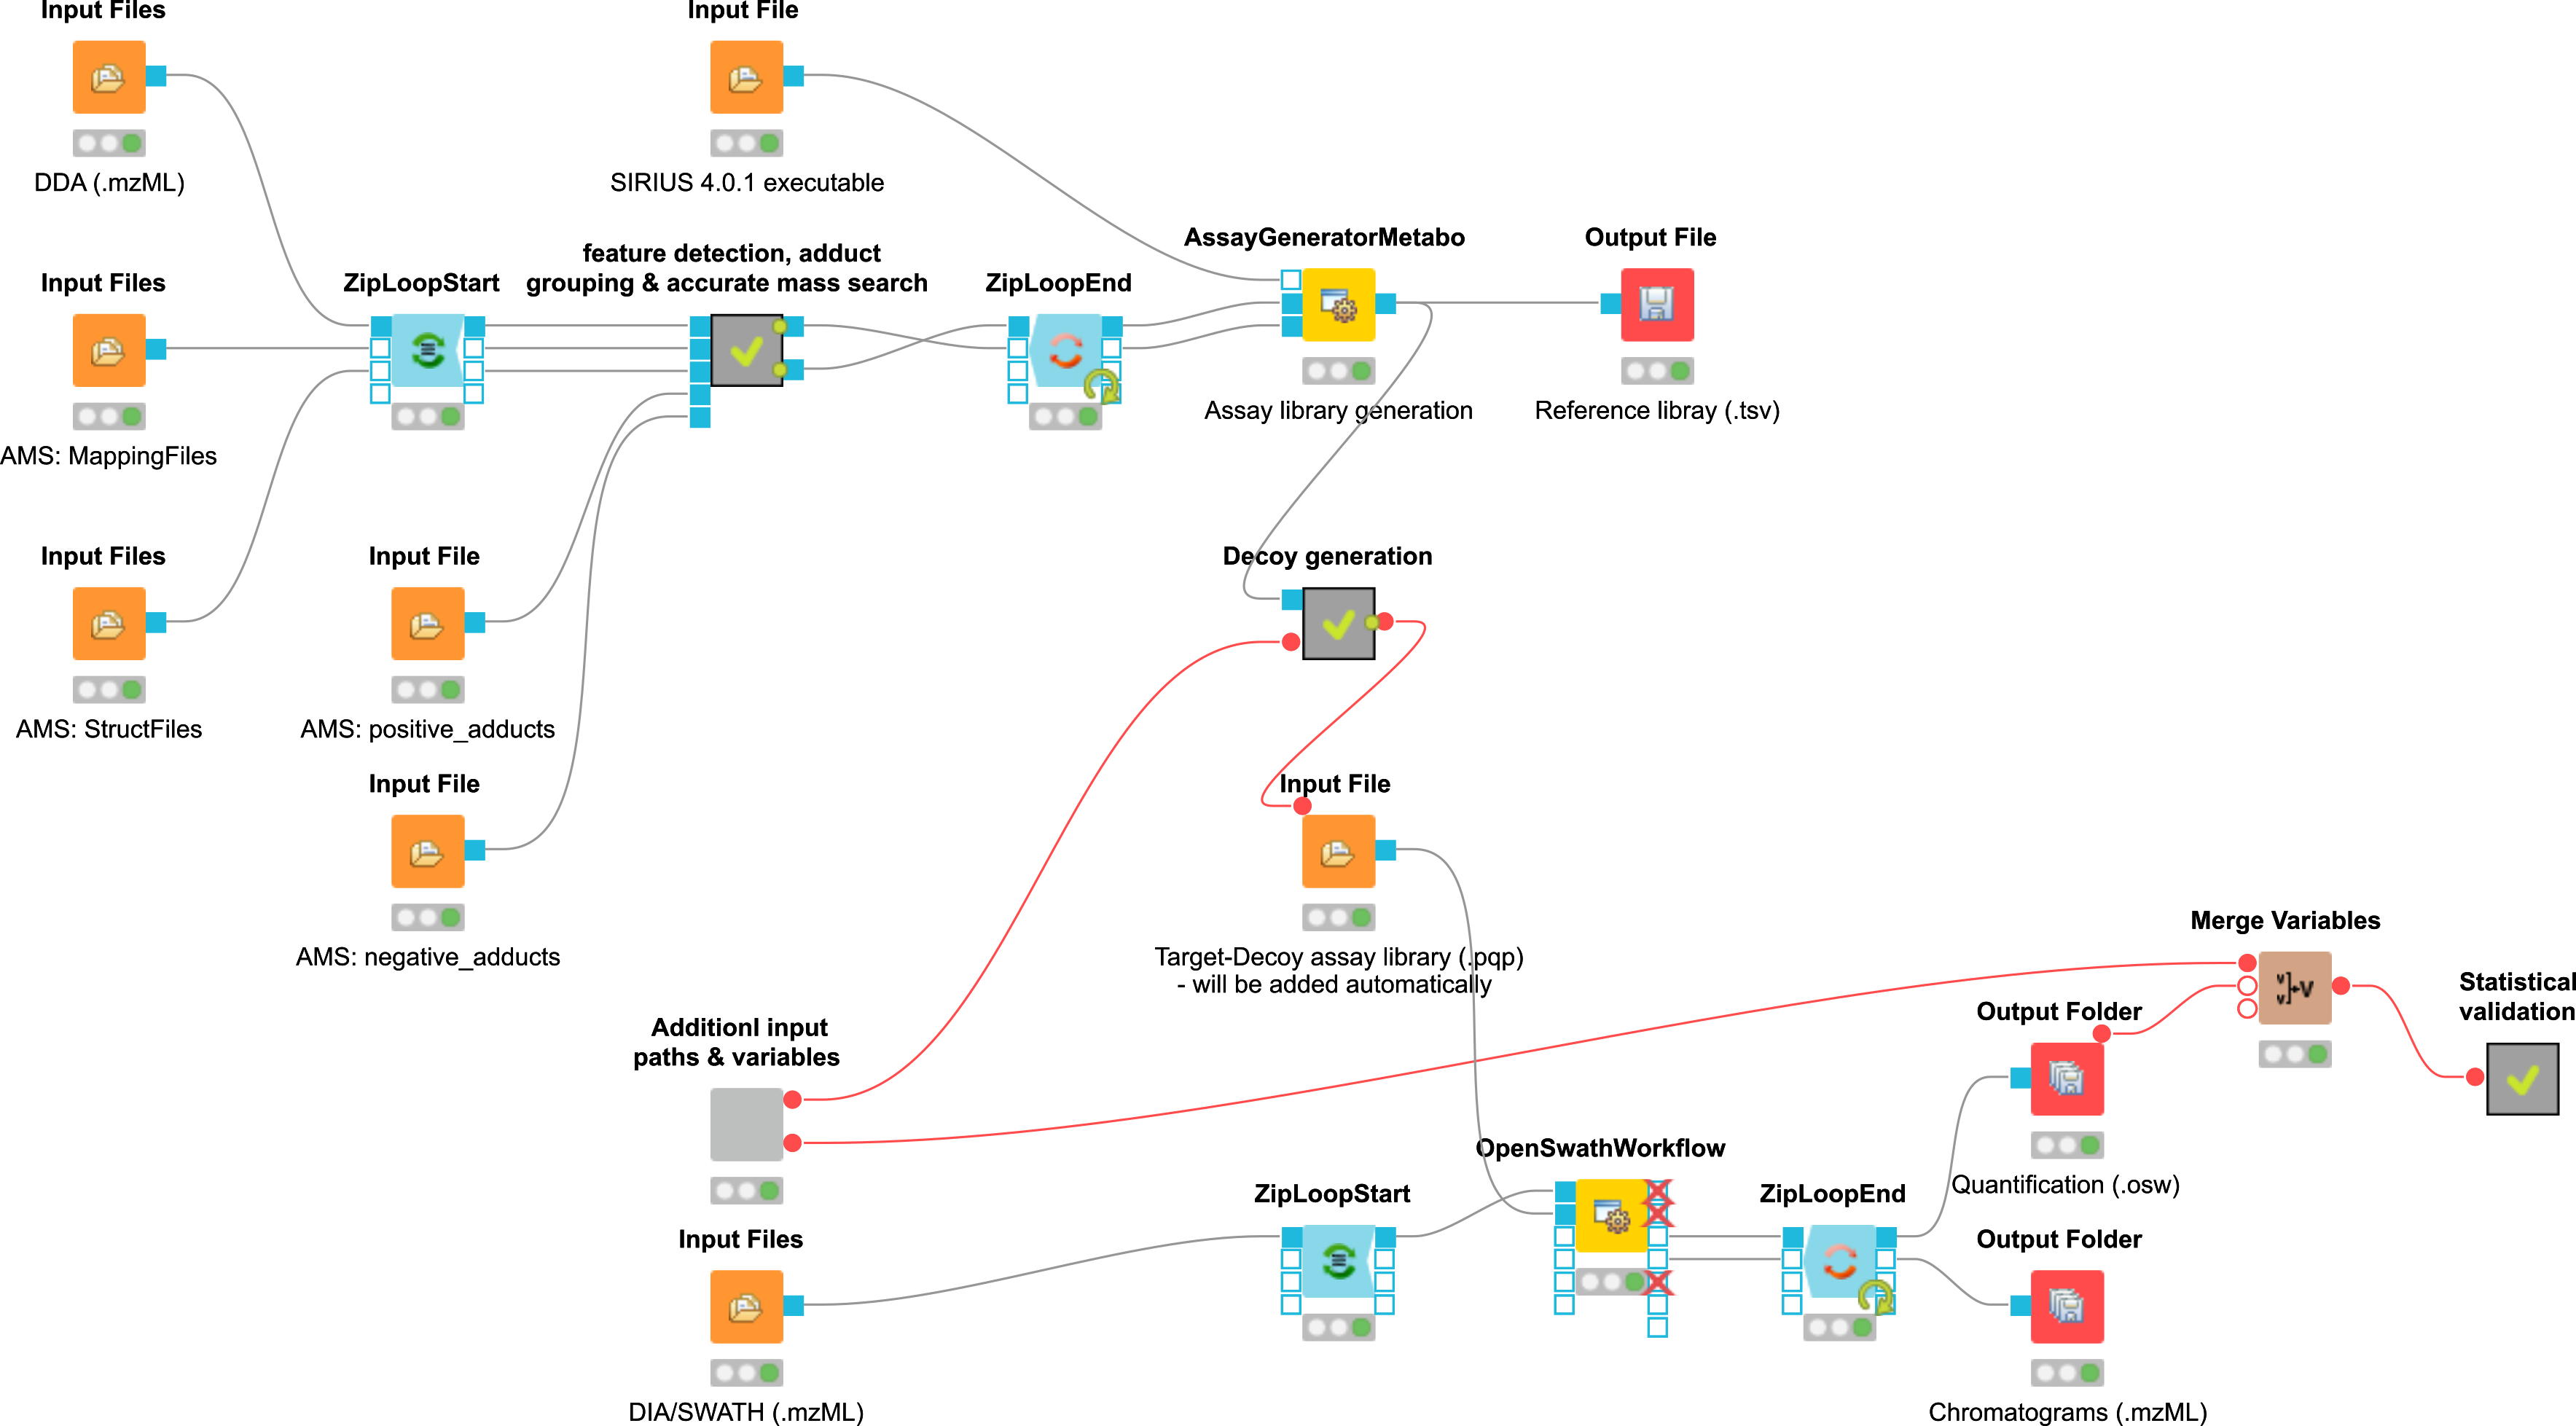
\includegraphics[width=0.95\textwidth]{graphics/openswathmetabo/oswm_example_wf.png}
  \caption{Example workflow for the usage of the DIAMetAlyzer Pipeline in KNIME}
  \label{fig:oswm_example_wf}
\end{figure}

\subsection{Run the Workflow}
These steps need to be followed to run the workflow successfully:

\begin{itemize}
\item Add DDA Input Files (.mzML).
\item Specify SIRIUS 4.0.1 executable.
\item Specify library files (mapping, struct) for \KNIMENODE{AccurateMassSearch}.
\item Add positive/negative adducts lists for \KNIMENODE{AccurateMassSearch}
\item Supply an output path for the SIRIUS workspace in the \KNIMENODE{AssayGeneratorMetabo}.
\item Specify additional paths and variables, such as an output path for the target-decoy assay library and a path to the pyprophet installation as well as decoy fragment mz filter (min/max).
\item Input DIA/SWATH files (.mzML).
\item Specify output path in the output folders.
\item Ready to go - run the workflow! 
\end{itemize}

\subsection{Important parameters}
\noindent Please have a look at the most important parameters, which should be tweaked to fit your data. In general, OpenMS has a lot of room for parameter optimization to best fit your chromatography and instrumental settings. \\

\noindent\KNIMENODE{\textbf{FeatureFinderMetabo}}:
\begin{center}
\begin{tabular*}{\textwidth}{ p{5.5cm}|p{10.5cm} }
\textbf{parameter} & \textbf{explanation} \\ \hline
\textit{noise\_threshold\_int} & Intensity threshold below which peaks are regarded as noise. \\
\textit{chrom\_fwhm} & Expected chromatographic peak width (in seconds). \\
\textit{mass\_error\_ppm} & Allowed mass deviation (in ppm) \\
%\textit{algorithm $\rightarrow$ common $\rightarrow$ noise\_threshold\_int} & Intensity threshold below which peaks are regarded as noise. \\
%\textit{algorithm $\rightarrow$ common $\rightarrow$ chrom\_fwhm} & Expected chromatographic peak width (in seconds). \\
%\hl{\textit{algorithm $\rightarrow$ mtd $\rightarrow$ mass\_error\_ppm}} & Allowed mass deviation (in ppm) \\
\end{tabular*}
\end{center}

\noindent\KNIMENODE{\textbf{MetaboliteAdductDecharger}}:
\begin{center}
\begin{tabular*}{\textwidth}{ p{5.5cm}|p{10.5cm} }
\textbf{parameter} & \textbf{explanation} \\ \hline
\textit{mass\_max\_diff} & Maximum allowed mass tolerance per feature.. \\
\textit{potential\_adducts} & Adducts used to explain mass differences - These should fit to the adduct list specified for AccurateMassSearch. \\
%\hl{\textit{algorithm $\rightarrow$ MetaboliteFeatureDeconvolution $\rightarrow$ mass\_max\_diff}} & Maximum allowed mass tolerance per feature. \\
%\hl{\textit{algorithm $\rightarrow$ MetaboliteFeatureDeconvolution $\rightarrow$ potential\_adducts}} & Adducts used to explain mass differences - These should fit to the adduct list specified for AccurateMassSearch. \\
\end{tabular*}
\end{center}

\noindent\KNIMENODE{\textbf{AccurateMassSearch}}:
\begin{center}
\begin{tabular*}{\textwidth}{ p{5.5cm}|p{10.5cm} }
\textbf{parameter} & \textbf{explanation} \\ \hline
\textit{mass\_error\_value} & Tolerance allowed for accurate mass search. \\
\textit{ionization\_mode} &  Positive or negative ionization mode. \\
\end{tabular*}
\end{center}

\noindent\KNIMENODE{\textbf{AssayGeneratorMetabo}}:
\begin{center}
\begin{tabular*}{\textwidth}{ p{5.5cm}|p{10.5cm} }
\textbf{parameter} & \textbf{explanation} \\ \hline
\textit{min\_transitions} & Minimal number of transitions (3). \\
\textit{max\_transitions} &  Maximal number of transitions (3). \\
\textit{transitions\_threshold} & Further transitions need at least x\% of the maximum intensity. \\
\textit{out\_workspace\_directory} & Output directory for SIRIUS workspace (Fragmentation Trees). \\
\textit{filter\_by\_num\_masstraces} &  Features have to have at least x MassTraces. To use this parameter feature\_only is neccessary. \\
\textit{precursor\_mass\_tolerance} & Tolerance window for precursor selection (Feature selection in regard to the precursor). \\
\textit{precursor\_rt\_tolerance} & Tolerance allowed for matching MS2 spectra depeding on the feature size (should be around the FWHM of the chromatograms). \\
\textit{profile} & Specify the used analysis profile (e.g. qtof). \\
\textit{elements} & Allowed elements for assessing the putative sumformula (e.g. CHNOP[5]S[8]Cl[1]). Elements found in the isotopic pattern are added automatically, but can be specified nonetheless. \\
\end{tabular*}
\end{center}

\noindent\KNIMENODE{\textbf{OpenSWATH}}:
\begin{center}
\begin{tabular*}{\textwidth}{ p{5.5cm}|p{10.5cm} }
\textbf{parameter} & \textbf{explanation} \\ \hline
\textit{rt\_extraction\_window} & Extract x seconds around this value. \\
\textit{rt\_normalization\_factor} &  Please use the range of your gradient e.g. 950 seconds. \\
\end{tabular*}
\end{center} 

\noindent If you are analysing a lot of big DIA mzML files $\approx$ 3-20GB per File, it makes sense to change how OpenSWATH processes the spectra. 

\begin{center}
\begin{tabular*}{\textwidth}{ p{5.5cm}|p{10.5cm} }
\textbf{parameter} & \textbf{explanation} \\ \hline
\textit{readOptions} & Set cacheWorkingInMemory - will cache the files to disk and read SWATH-by-SWATH into memory\\
\textit{tempDirectory} &  Set a directory, where cached mzMLs are stored (be aware that his directory can be quite huge depending on the data). \\
\end{tabular*}
\end{center} 

\noindent In the workflow pyprophet is called after OpenSWATH, it merges the result files, which allows to get enough data for the model training. 

\begin{lstlisting}
pyprophet merge  --template path_to_target-decoy_assay_library.pqp --out merged.osw  ./*.osw
\end{lstlisting}

\noindent Afterwards, the results are scored using the MS1 and MS2 levels and filter for metabolomics scores, which have a low correlation. 

\begin{lstlisting}
pyprophet score --in  merged.osw  --out  scored.osw --level ms1ms2 --ss_main_score "var_isotope_correlation_score" --ss_score_filter metabolomics
\end{lstlisting}
\noindent Export the non filtered results: 

\begin{lstlisting}
pyprophet export-compound --in scored.osw --out scored + "_pyprophet_nofilter_ms1ms2.tsv" 
--max_rs_peakgroup_qvalue 1000.0
\end{lstlisting}
\noindent Please see the workflow for actual parameter values used for the benchmarking dataset. \\


\noindent  The workflow can be used without any identification (remove \KNIMENODE{AccurateMassSearch}). Here, all features (known\_unknowns) are processed. The assay library is constructed based on the chemical composition elucidated via the fragment annotation. Quantification is possible, unfortunately the decoy generation and FDR estimation for this case is not yet available. 


